\section{Наблюдатель полного порядка}

Заданы матрицы системы:
\[
A = \begin{bmatrix}
    25 & 40 & 18 & -30 \\
    -17 & -27 & -13 & 20 \\
    -10 & -14 & -7 & 14 \\
    -7 & -10 & -6 & 9
\end{bmatrix}, \quad
C = \begin{bmatrix}
    1 & 1 & 1 & -1
\end{bmatrix}.
\]

Рассмотрим следующие спектры сходимости для синтеза наблюдателя:
\[
    \sigma_1 = \{-2, -2, -2, -2\}, \quad
    \sigma_2 = \{-2, -20, -200, -2000\}, \quad
    \sigma_3 = \{-2 \pm 3i, -2 \pm 4pti\}.
\]

\subsection{Исследование наблюдаемости системы}

Найдём собственные числа матрицы $A$:
\[
    \lambda_{1,2} = \pm 3i, \quad \lambda_{3,4} = \pm i.
\]

Все собственные числа являются комплексными, что указывает на колебательный характер вектора состояния.

Матрица наблюдаемости системы:
\[
V = \begin{bmatrix}
    C \\
    CA \\
    CA^2 \\
    CA^3
\end{bmatrix} =
\begin{bmatrix}
    1 & 1 & 1 & -1 \\
    5 & 9 & 4 & -5 \\
    -33 & -49 & -25 & 41 \\
    -29 & -57 & -28 & 29
\end{bmatrix}.
\]

Ранг матрицы $V$ равен 4, что соответствует полной размерности системы. Согласно критерию Калмана, система является \textbf{полностью наблюдаемой}. Это также означает, что все собственные числа наблюдаемы, и система является \textbf{обнаруживаемой}.

Рассмотрим несколько вариантов синтеза наблюдателей с различными спектрами сходимости.


\subsection{Первый спектр}

Рассмотрим систему с наблюдателем полного порядка, заданную уравнениями:
\[
\begin{cases}
    \dot{x} = Ax + Bu, \\
    y = Cx,
\end{cases}
\]
\[
\begin{cases}
    \dot{\hat{x}} = A\hat{x} + Bu + L(\hat{y} - y), \\
    \hat{y} = C\hat{x}.
\end{cases}
\]

Для синтеза наблюдателя должны выполняться следующие условия:
\begin{enumerate}
    \item Спектры матриц $A$ и $G$ не пересекаются: $\sigma(A) \cap \sigma(G) = \emptyset$.
    \item Пара $(G, Y)$ является управляемой.
    \item Пара $(C, A)$ является наблюдаемой.
\end{enumerate}


\subsubsection{Алгоритм синтеза наблюдателя}

\begin{enumerate}
    \item Выбираем матрицу $G \in \mathbb{R}^{n \times n}$ с желаемым спектром $\sigma(G)$.
    \item Выбираем матрицу $Y \in \mathbb{R}^{n \times k}$ так, чтобы пара $(G, Y)$ была управляемой.
    \item Находим матрицу $Q \in \mathbb{R}^{n \times n}$ как решение уравнения Сильвестра:
    \[
    GQ - QA = YC.
    \]
    \item Вычисляем матрицу коррекции наблюдателя:
    \[
    L = Q^{-1}Y.
    \]
\end{enumerate}

Для желаемого спектра $\sigma_1 = \{-2, -2, -2, -2\}$ выберем:
\[
G = \begin{bmatrix}
    -2 & 1 & 0 & 0 \\
    0 & -2 & 1 & 0 \\
    0 & 0 & -2 & 1 \\
    0 & 0 & 0 & -2
\end{bmatrix}, \quad
Y = \begin{bmatrix}
    1 \\
    1 \\
    1 \\
    1
\end{bmatrix}.
\]

После вычислений получаем матрицу коррекции наблюдателя:
\[
L = \begin{bmatrix}
    -4.29 \\
    3.04 \\
    -13.83 \\
    -7.08
\end{bmatrix}.
\]

Собственные числа матрицы наблюдателя $(A + LC)$:
\[
\sigma_{\text{obsv}} \approx \{-2, -2, -2, -2\}.
\]

\subsubsection{Моделирование системы}

Проведём моделирование и построим графики:
\begin{enumerate}
    \item Сравнительный график сходимости вектора состояния системы $x(t)$ и наблюдателя $\hat{x}(t)$.
    \item График ошибки наблюдателя $e(t) = x(t) - \hat{x}(t)$.
\end{enumerate}

\begin{figure}[H]
    \centering
    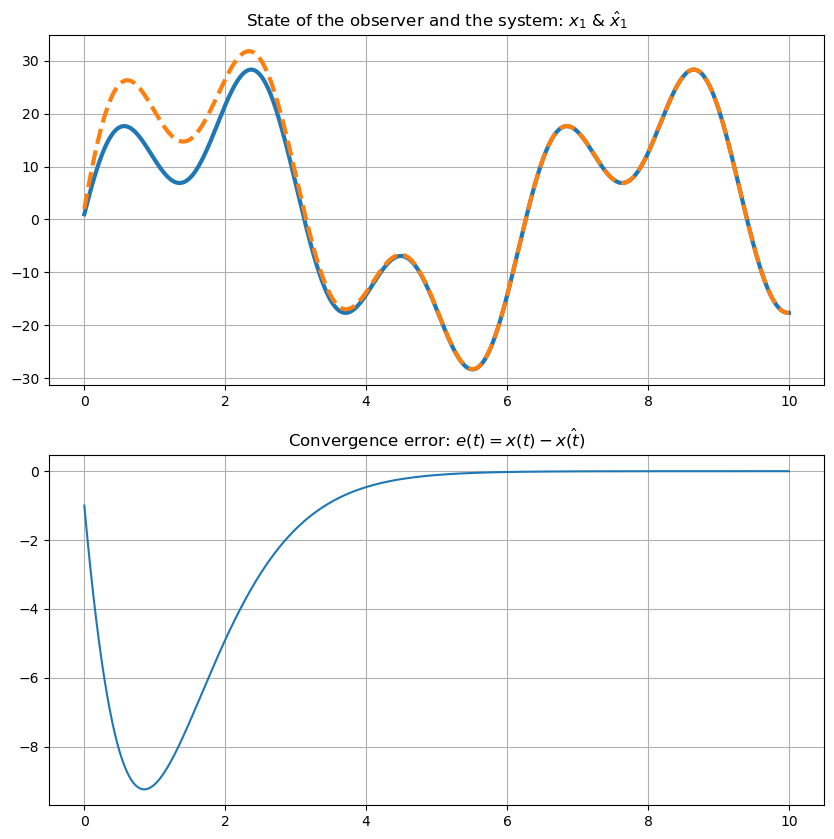
\includegraphics[width=0.6\textwidth]{../../plots/task_2_1.png}
    \caption{Состояние системы и ошибка сходимости}
    \label{fig:task_2_state_error_system_1_1}
\end{figure}

\begin{figure}[H]
    \centering
    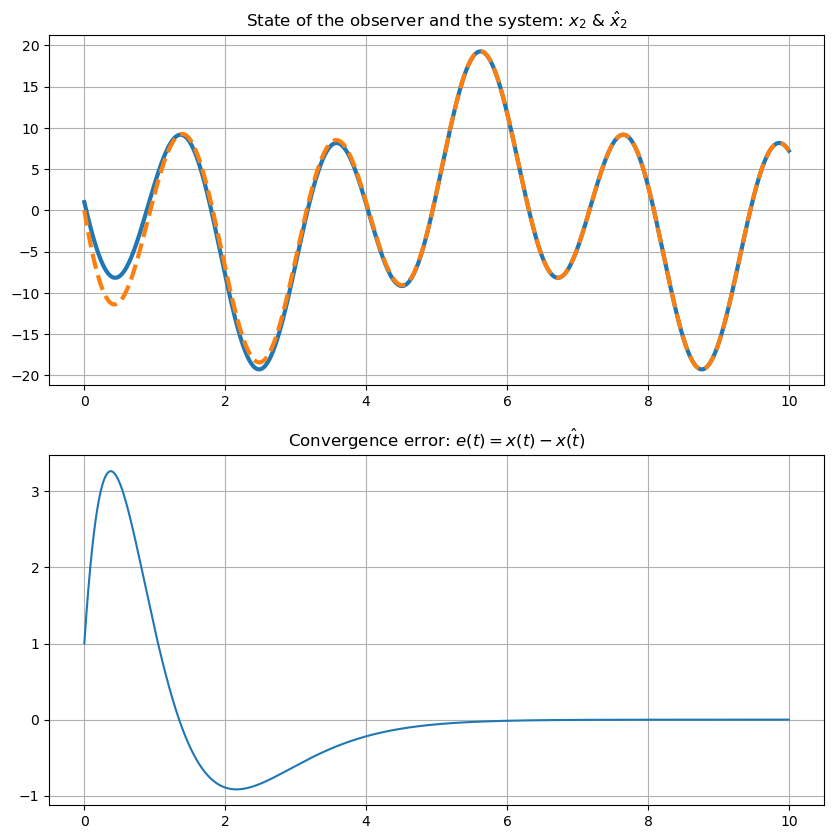
\includegraphics[width=0.6\textwidth]{../../plots/task_2_2.png}
    \caption{Состояние системы и ошибка сходимости}
    \label{fig:task_2_state_error_system_1_2}
\end{figure}

\begin{figure}[H]
    \centering
    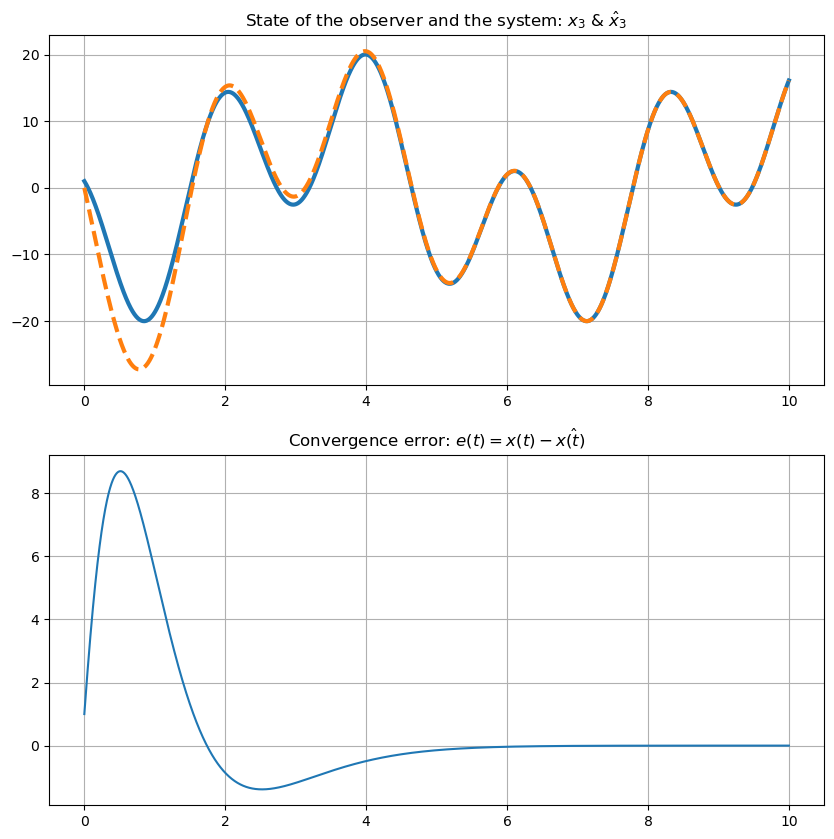
\includegraphics[width=0.6\textwidth]{../../plots/task_2_3.png}
    \caption{Состояние системы и ошибка сходимости}
    \label{fig:task_2_state_error_system_1_3}
\end{figure}

\begin{figure}[H]
    \centering
    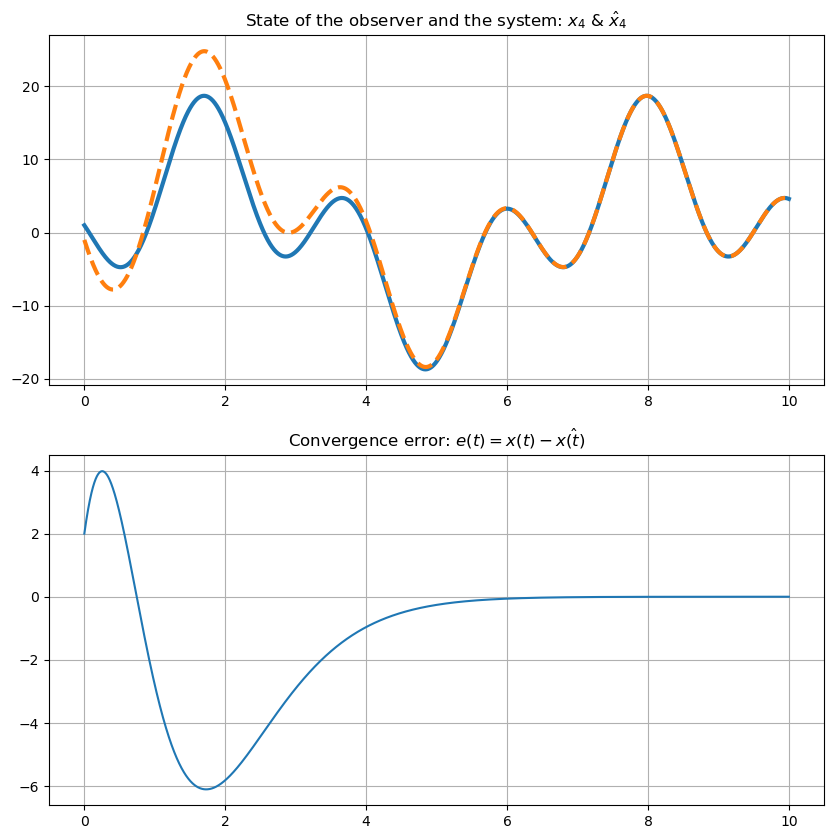
\includegraphics[width=0.6\textwidth]{../../plots/task_2_4.png}
    \caption{Состояние системы и ошибка сходимости}
    \label{fig:task_2_state_error_system_1_4}
\end{figure}


\subsection{Второй спектр}

Для желаемого спектра $\sigma_2 = \{-2, -20, -200, -2000\}$ выберем:
\[
G = \begin{bmatrix}
    -2 & 0 & 0 & 0 \\
    0 & -20 & 0 & 0 \\
    0 & 0 & -200 & 0\\
    0 & 0 & 0 & -2000\end{bmatrix}, \quad
Y = \begin{bmatrix}
    1 \\
    1 \\
    1 \\
    1
\end{bmatrix}.
\]

После вычислений получаем матрицу коррекции наблюдателя:
\[
L = 10^6\begin{bmatrix}
    -5.49 \\
    5.0 \\
    -2.44 \\
    -2.56ы
\end{bmatrix}.
\]

Собственные числа матрицы наблюдателя $(A + LC)$:
\[
\sigma_{\text{obsv}} \approx \{-2, -20, -200, -2000\}.
\]

\subsubsection{Моделирование системы}

Проведём моделирование и построим графики:
\begin{enumerate}
    \item Сравнительный график сходимости вектора состояния системы $x(t)$ и наблюдателя $\hat{x}(t)$.
    \item График ошибки наблюдателя $e(t) = x(t) - \hat{x}(t)$.
\end{enumerate}

\begin{figure}[H]
    \centering
    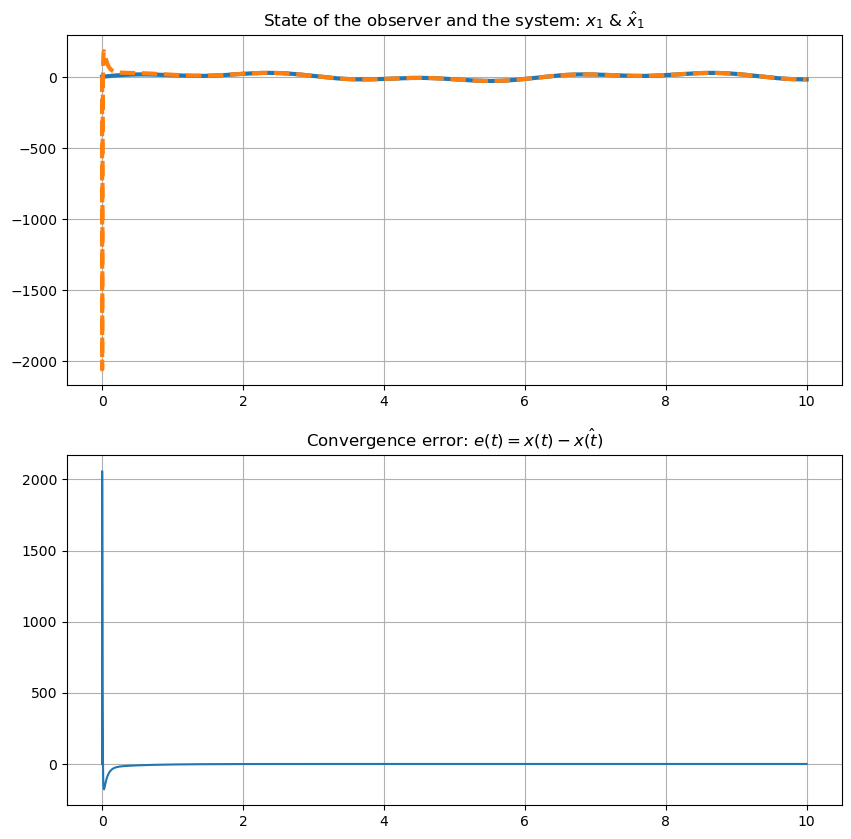
\includegraphics[width=0.6\textwidth]{../../plots/task_2_5.png}
    \caption{Состояние системы и ошибка сходимости}
    \label{fig:task_2_state_error_system_2_1}
\end{figure}

\begin{figure}[H]
    \centering
    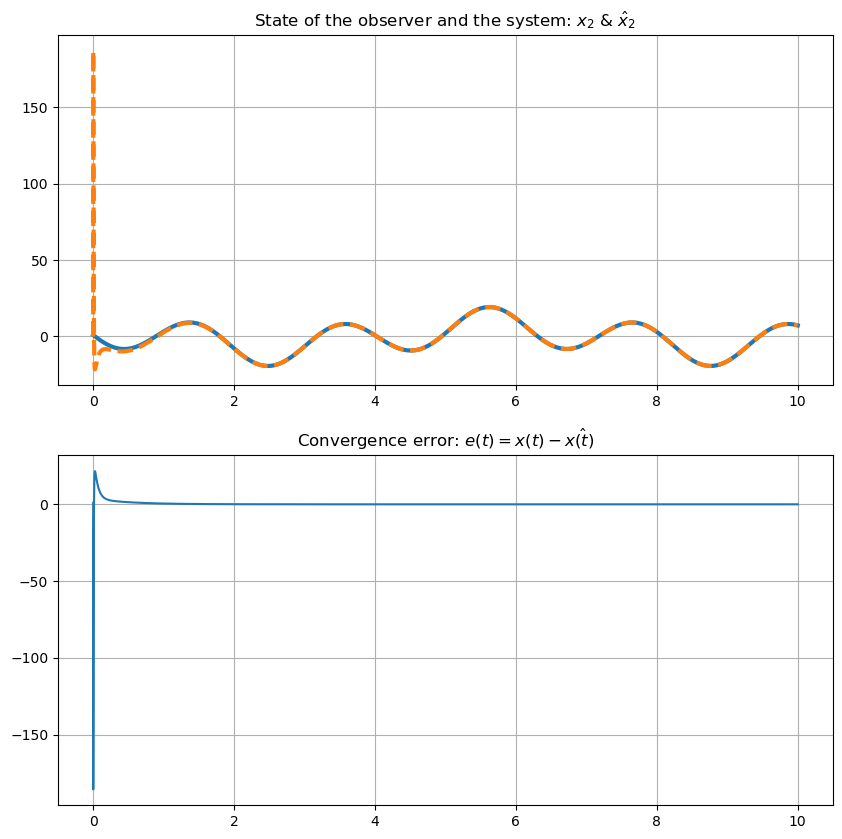
\includegraphics[width=0.6\textwidth]{../../plots/task_2_6.png}
    \caption{Состояние системы и ошибка сходимости}
    \label{fig:task_2_state_error_system_2_2}
\end{figure}

\begin{figure}[H]
    \centering
    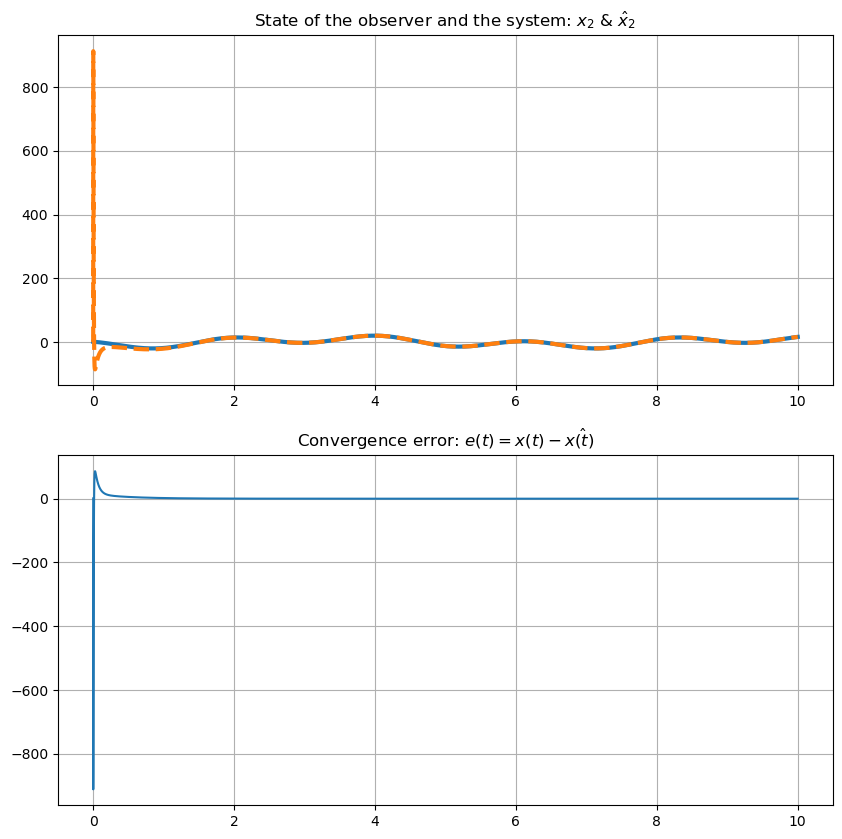
\includegraphics[width=0.6\textwidth]{../../plots/task_2_7.png}
    \caption{Состояние системы и ошибка сходимости}
    \label{fig:task_2_state_error_system_2_3}
\end{figure}

\begin{figure}[H]
    \centering
    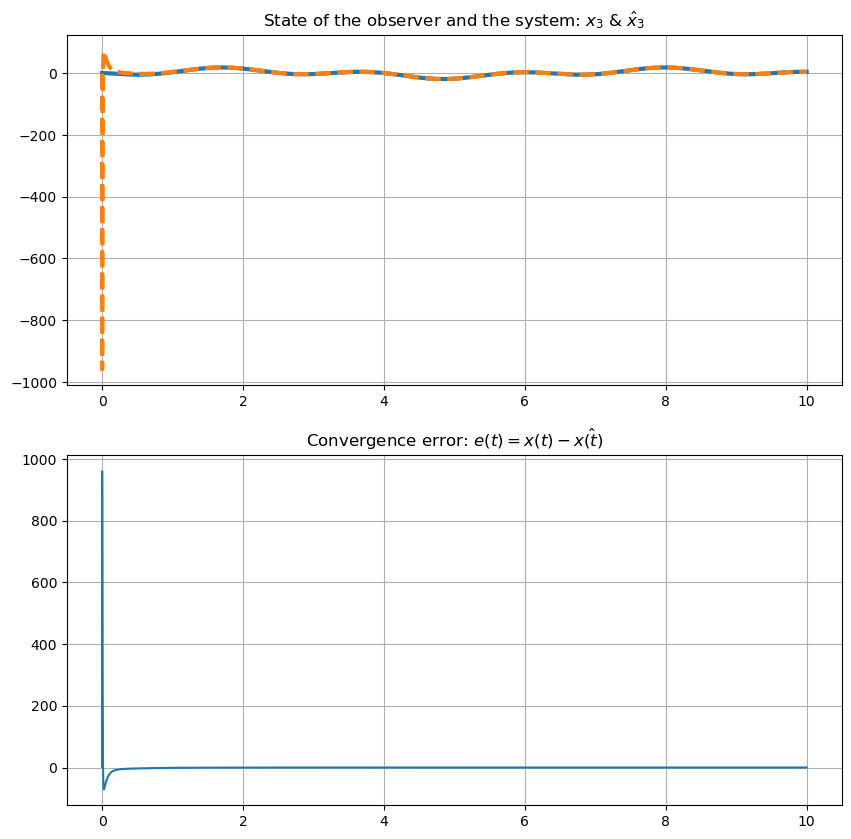
\includegraphics[width=0.6\textwidth]{../../plots/task_2_8.png}
    \caption{Состояние системы и ошибка сходимости}
    \label{fig:task_2_state_error_system_2_4}
\end{figure}


\subsection{Третий спектр}

Для желаемого спектра $\sigma_3 = \{-2 \pm 3j, -2 \pm 4j\}$ выберем:
\[
G = \begin{bmatrix}
    -2 & 3 & 0 & 0 \\
    -3 & -2 & 0 & 0 \\
    0 & 0 & -2 & 4 \\
    0 & 0 & -4 & -2 \end{bmatrix}, \quad
Y = \begin{bmatrix}
    1 \\
    1 \\
    1 \\
    1
\end{bmatrix}.
\]

После вычислений получаем матрицу коррекции наблюдателя:
\[
L = \begin{bmatrix}
    -72.33 \\
    3.83 \\
    14.33 \\
    -46.17
\end{bmatrix}.
\]

Собственные числа матрицы наблюдателя $(A + LC)$:
\[
\sigma_{\text{obsv}} \approx \{-2 \pm 3j, -2 \pm 4j\}.
\]

\subsubsection{Моделирование системы}

Проведём моделирование и построим графики:
\begin{enumerate}
    \item Сравнительный график сходимости вектора состояния системы $x(t)$ и наблюдателя $\hat{x}(t)$.
    \item График ошибки наблюдателя $e(t) = x(t) - \hat{x}(t)$.
\end{enumerate}

\begin{figure}[H]
    \centering
    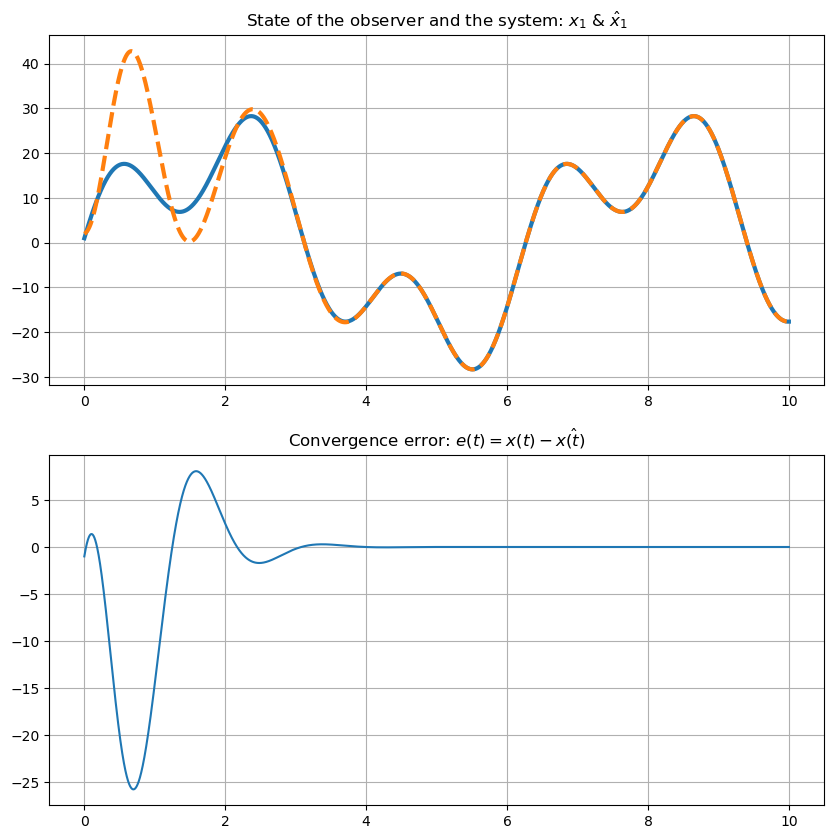
\includegraphics[width=0.6\textwidth]{../../plots/task_2_9.png}
    \caption{Состояние системы и ошибка сходимости}
    \label{fig:task_2_state_error_system_3_1}
\end{figure}

\begin{figure}[H]
    \centering
    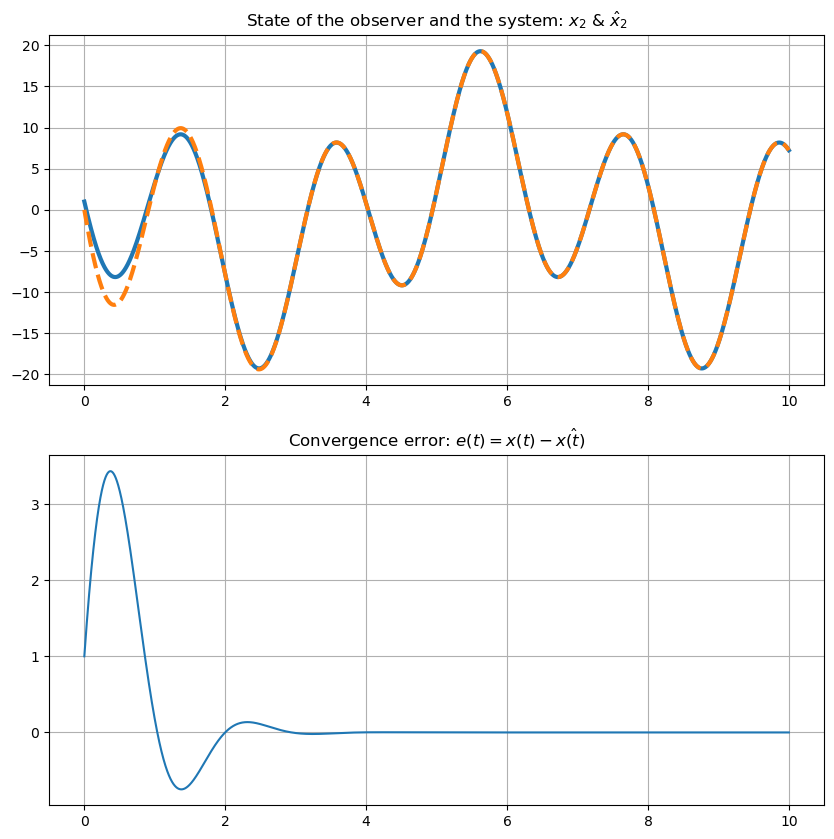
\includegraphics[width=0.6\textwidth]{../../plots/task_2_10.png}
    \caption{Состояние системы и ошибка сходимости}
    \label{fig:task_2_state_error_system_3_2}
\end{figure}

\begin{figure}[H]
    \centering
    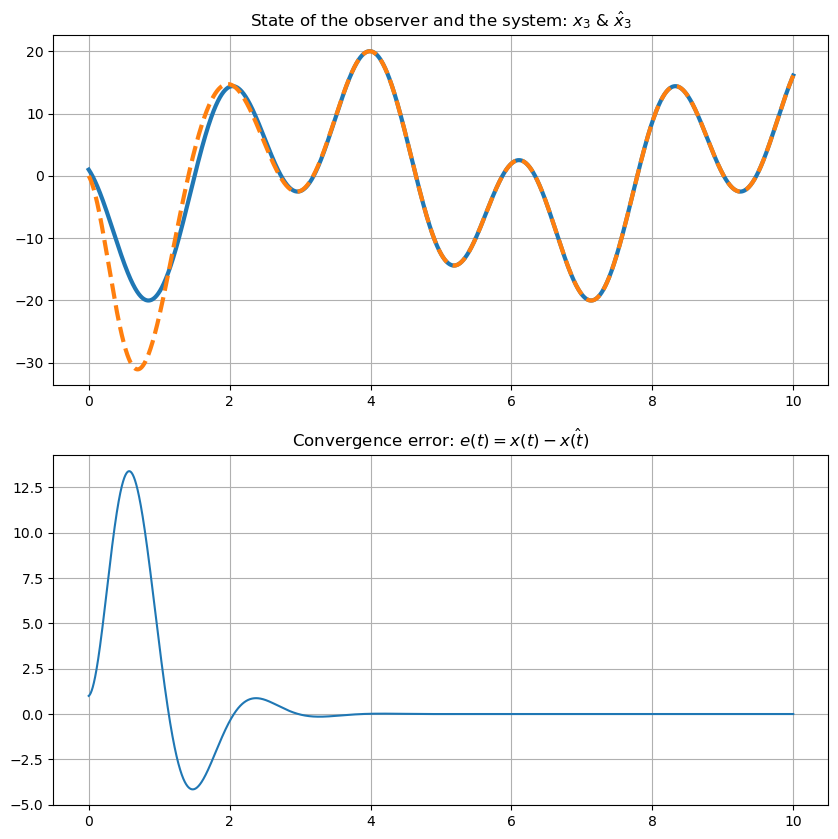
\includegraphics[width=0.6\textwidth]{../../plots/task_2_11.png}
    \caption{Состояние системы и ошибка сходимости}
    \label{fig:task_2_state_error_system_3_3}
\end{figure}

\begin{figure}[H]
    \centering
    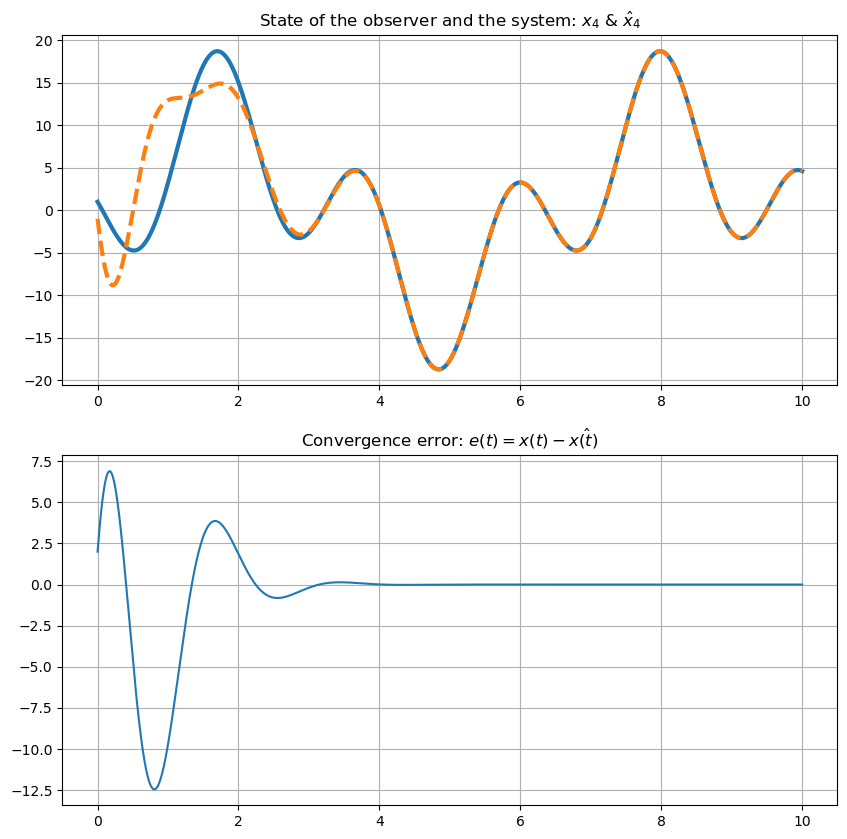
\includegraphics[width=0.6\textwidth]{../../plots/task_2_12.png}
    \caption{Состояние системы и ошибка сходимости}
    \label{fig:task_2_state_error_system_3_4}
\end{figure}

\subsection{Сравнение выбора спектра для синтеза наблюдателя}

Мы наблюдаем процессы, аналогичные синтезу модального регулятора: выбор мод наблюдателя напрямую влияет на характер его сходимости к истинной системе.

\subsubsection{Первый случай}
Спектр выбран с относительно небольшими модами. В результате матрица коррекции $L$ имеет умеренные значения, что приводит к значительному перерегулированию (видно на графике ошибки) при сравнительно небольшом времени переходного процесса.

\subsubsection{Второй случай}
Спектр выбран с большими модами, что обеспечивает агрессивную сходимость. Перерегулирование практически отсутствует, а время переходного процесса крайне мало. Однако в реальных физических системах такая быстрая и резкая сходимость маловероятна из-за наличия шумов. Для фильтрации шумов требуется время на сбор и обработку данных.

\subsubsection{Третий случай}
Спектр включает колебательные моды, что приводит к переходному процессу с большим перерегулированием по сравнению с первым случаем. Однако время переходного процесса значительно сокращается.


\subsection{Вывод}
Мы работали с \textbf{полностью наблюдаемой системой}, что было подтверждено с использованием критерия Калмана. Синтез наблюдателей позволяет реализовать различные характеры сходимости. Для этого был синтезирован \textbf{модальный наблюдатель} с использованием уравнения Сильвестра. Проведённые моделирования с различными наблюдателями показали, что все они обеспечивают сходимость к исходной системе, но с разным качеством переходного процесса: временем сходимости и уровнем перерегулирования.